\documentclass[11pt]{article}
\input{/Users/markwang/.preamble}

\title{CSC458 Problem Set 1}

\begin{document}

\maketitle

\section*{chapter 1}

\textbf{13} 1-Gbps P2P link from earth to moon. Distance 385000km. Data transmit at speed of light 

\begin{enumerate}
    \item Minimum RTT is at least the propagation delay
    \[
        RTT = \frac{2\times 385000000 m}{3\times 10^8 m/s} = 2.57s
    \]
    \item Using the RTT as the delay, calculate the delay $\times$ bandwidth product for the link.
    \[
        delay \times bandwidth = 2.57s \times 10^9 bit/s = 2.57 Gb
    \]
    \item The delay-bandwidth product is equivalent to the amount of data that sender is required to send before receiving the receiver's acknowledgement. This is an important parameter in design of protocols like TCP. Have to consider the fact that protocol have the highest throughput only if the sender send sufficiently large (referencing delay-bandwidth product) amount of data. 
    \item Assume request has negligible transmission time. 
    \[
        transferTime = RTT + transferSize/bandwidth = 2.57s + 
        \frac{25\times 8 \times 10^6 bits}{10^9 bit/s} = 2.57s + 0.2s = 2.77s 
    \]
\end{enumerate}
\textbf{16} Calculate the latency (from first bit sent to last bit received) for the following

\begin{enumerate}
    \item 100-Mbps with a single store-and-forward switch in path and packet size of 12000bits. Assume each link has propagation delay of 10 $\mu s$ and switch begins retransmitting immediately after receiving packet\\ 
    \[
        \text{transmission delay} = \frac{12000bits}{10^8 bits/s} = 120 \mu s
    \]
    \[
        delay = 2\times \text{transmission delay} + 2\times \text{propagation delay} = 240\mu s + 20\mu s = 260 \mu s
    \]
    \item same as 1 but 3 switches
    \[
        delay = 4\times \text{transmission delay} + 4\times \text{propagation delay} = 520\mu s
    \]
    \item Same as 1. But switch implements cut through switching. Able to retransmit the packet after the first 200bits are received
    \[
        \text{switch's delay} = \frac{200 bits}{10^8 bits/s} = 2 \mu s
    \]
    \[
        delay = \text{switch's delay} + 2\times \text{propagation delay} + \text{transmission delay} = 2\mu s + 20\mu s + 120 \mu s= 142 \mu s
    \]
    Note although we reduced switch delay to $4\mu s$, we still have 1 transmission delay to wait for the last bit to arrive
\end{enumerate}
\textbf{19} Calculate delay-bandwidth product for links, Use one-way delay, measured from first bit sent to first bit received
\begin{enumerate}
    \item 100Mbps ethernet with delay of 10 $\mu s$
    \[
        delay\times bandwidth = 10\mu s \times 10^8 bits/s = 1000 bits
    \]
    \item 100Mbps ethernet with 3 single store-and-forward switch, a packet size of 12000bits, and $10 \mu s$ propagation delay \\
    Use result from \textbf{16.2}\\
    Since we are concerned with time between first bit sent and first bit received
    \[
        delay = 3\times \text{transmission delay} + 4\times \text{propagation delay} = 400\mu s
    \]
    \[
        delay\times bandwidth = 400\mu s \times 10^8 bits/s = 4\times 10^4 bits
    \]
    \item 1.5Mbps T1 link, with transcontinental one-way delay of $50ms$
    \[
        delay\times bandwidth = 50ms \times 1.5\times 10^6 bits/s = 7.5 \times 10^4 bits
    \]
    \item 1.5Mbps T1 link between 2 gounrdtation via a satellite 35900km high. Only delay is propagation delay from earth to satellite and back 
    \[
        delay = \frac{35900000m}{3\times 10^8 m/s} = 0.24s
    \]
    \[
        delay\times bandwidth = 0.24s \times 1.5\times 10^6 bits/s = 3.6\times 10^5 bits/s
    \]
\end{enumerate}
\textbf{26} Calculate bandwidth necessary for transmitting in real time
\begin{enumerate}
    \item Video at $640\times 480$ 3 bytes/pixel, 30frames/s 
    \[
        bandwidth = 640\times 480 \times 3 \times 30 Bps = 27.6MB/s
    \]
    \item Video at $160\times 120$ 1 bytes/pixel, 5frames/s 
    \[
        bandwidth = 160\times 120 \times 1 \times 5 Bps = 96KB/s
    \]
    \item CD ROM assume 1 CD holds 75min worth and take 650MB
    \[
        bandwidth = \frac{650MB}{75min} = 144KB/s
    \]
    \item Fax $8\times 10$ inch black-and-white (1-bit/pixel) image at resolution of 72pixels/inch. How long would this take over a 14.4kbps modem
    \[
        size = 8\times 10 \times 72 \times 72 bits= 414720 bits
    \]
    \[
        time = \frac{414720 bits}{14400 bits/s} = 28.8s 
    \]
\end{enumerate}




\section*{chapter 2}

\textbf{17} Show that the Internet checksum can be computed by first taking the 32-bit ones complement sum of the buffer in 32-bit units, then taking the 16-bit ones complement sum of the upper and lower halfwords, and finishing as before by complementing the result. (To take a 32-bit ones complement sum on 32-bit twos complement hardware, you need access to the “overflow” bit.)
\begin{solution}
    Note that in ones complement addition, if carry occurs, the resulting sum is incremented by one to account for the carry. Conceptually, in taking 32-bit one complement sum buffer, the carries of the lower halfword is carried over to the least significant bits of the higher halfword and the carries of the higher halfword is carried over to the least significant bits of the lower halfword. Conceptually this is equivalenet to calculate 2 checksums (that skips 16-bits for each addition) where the carries are accumulated in the opposing checksum (i.e. checksum $X$'s carry makes checksum $Y$ increment by 1). Then ones complement addition of upper and lower 16bit halfword is equivalent to summing up two checksums, whose ones complement gives the Internet checksum
\end{solution}
\textbf{18}  Suppose we want to transmit the message $11100011$ and protect it from errors using the CRC polynomial $x^3 + 1$.
\begin{enumerate}
    \item Use polynomial long division to determine the message that should be transmitted.
    \begin{center}
        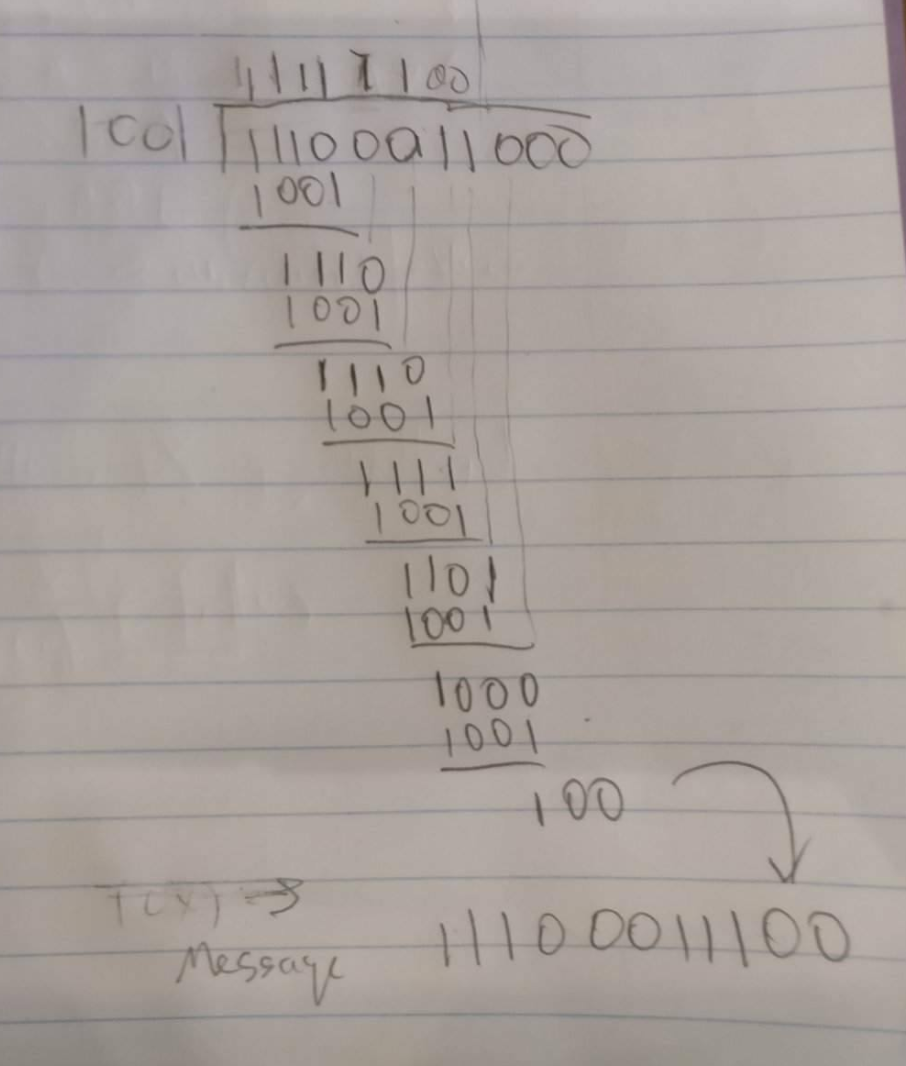
\includegraphics[scale=0.4]{2_18_1}        
    \end{center}
    \item Suppose the left most bit of the message is inverted due to noise on the transmission link. What is the result of the receiver’s CRC calculation? How does the receiver know that an error has occurred?
    \begin{center}
        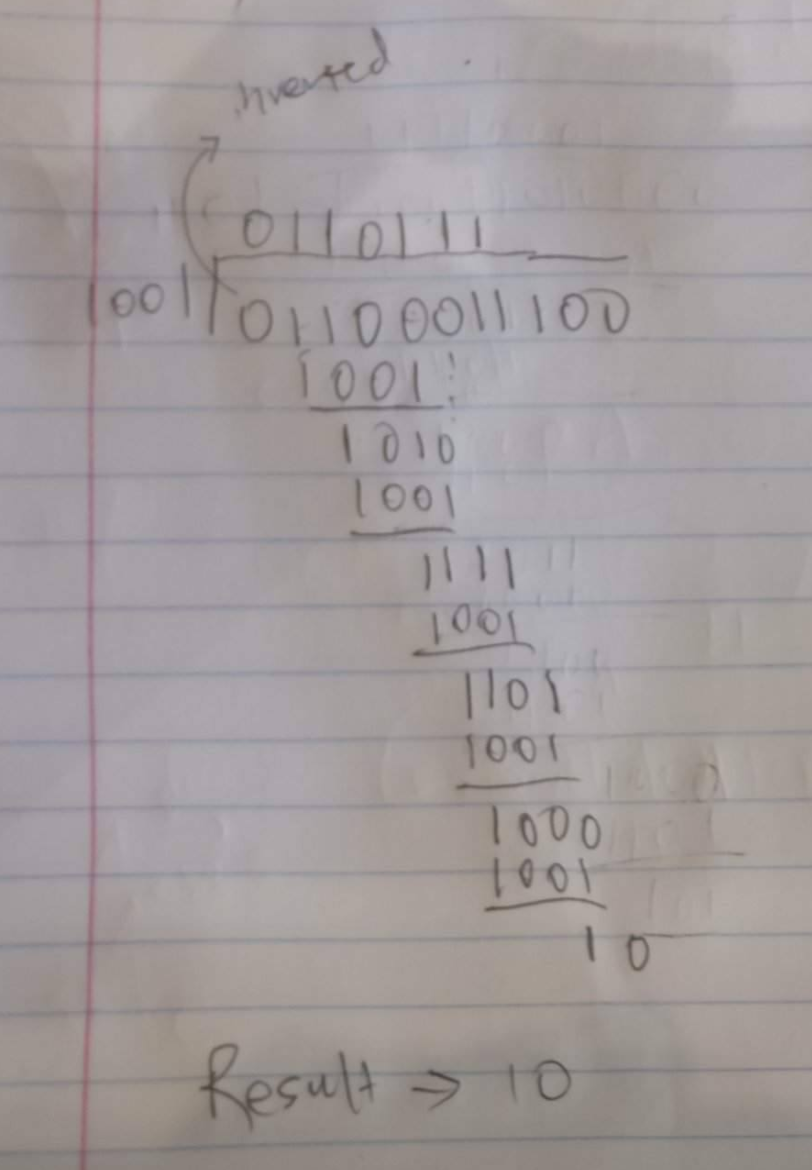
\includegraphics[scale=0.4]{2_18_2}        
    \end{center}
    The receiver knows that error occurs because the transmitted message is not divisible by $C(x)$, and yield a remainder $10$.
\end{enumerate}


\textbf{46} Suppose $A$, $B$, and $C$ all make their first carrier sense,as part of an attempt to transmit, while a fourth station D is transmitting. Draw a timeline showing one possible sequence of transmissions, attempts, collisions, and exponential backoff choices. Your timeline should also meet the following criteria: (i) initial transmission attempts should be in the order A, B, C but successful transmissions should be in the order C, B, A, and (ii) there should be at least four collisions.


\begin{solution}
Steps are given as 
\begin{enumerate}
    \item A, B, C tries to start transmission, in this order, and finds line busy and starts waiting. 
    \item When D finishes, A, B, C all tries to start to transmit. Collision happens. $k \subseteq \{0,1\}$ as A,B,C all experienced 1 collision. Suppose $k_A=1$, $k_B=1$, and $k_C =0$, C starts transmitting as line is idle 
    \item after 1 time slot, A, B finds line busy and wait until C is finished transmitting. A, B both attempts to transmit, collision happens., $k\subseteq \{ 0,1,2,3\}$. Suppose $k_A=1$, $k_B=1$, 
    \item After 1 time slot, both A and B tries transmitting again, collision happens again. $k\subseteq \{0, \cdots, 7\}$. Suppose this time $k_A=1$, $k_B=1$
    \item After 1 time slot, both A and B tries transmitting agian, collision happens again. $k\subseteq \{0. \cdots, 15\}$. Suppose this time $k_A=8$, $k_B=0$. B starts transmitting on the idle line immediately
    \item After 8 time slot, A starts transmitting or wait for B to finish before transmitting when the line becomes idle 
\end{enumerate}
\end{solution}



\section*{Chapter 3}


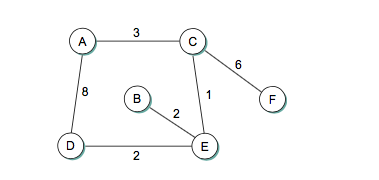
\includegraphics{ch3_3}\\
\textbf{3} For the network given in Figure3.45, give the datagram forwarding table for each node. The links are labeled with relative costs; your tables should forward each packet via the lowest-cost path to its destination.

\begin{solution}
    $A$
    \begin{center}
        \begin{tabular}{ |c|c| } 
        Destination & Next Node \\ 
        \hline  
        B & C  \\ 
        C & C  \\ 
        D & C  \\ 
        E & C  \\ 
        F & C  \\ 
        \end{tabular}
    \end{center}
    $B$
    \begin{center}
        \begin{tabular}{ |c|c| } 
        Destination & Next Node \\ 
        \hline  
        A & E  \\ 
        C & E  \\ 
        D & E  \\ 
        E & E  \\ 
        F & E  \\ 
        \end{tabular}
    \end{center}
    $C$
    \begin{center}
        \begin{tabular}{ |c|c| } 
        Destination & Next Node \\ 
        \hline  
        A & A  \\ 
        B & E  \\ 
        D & E  \\ 
        E & E  \\ 
        F & F  \\ 
        \end{tabular}
    \end{center}
    $D$
    \begin{center}
        \begin{tabular}{ |c|c| } 
        Destination & Next Node \\ 
        \hline  
        A & E  \\ 
        B & E  \\ 
        C & E  \\ 
        E & E  \\ 
        F & E  \\ 
        \end{tabular}
    \end{center}
    $E$
    \begin{center}
        \begin{tabular}{ |c|c| } 
        Destination & Next Node \\ 
        \hline  
        A & C  \\ 
        B & B \\ 
        C & C  \\ 
        D & D  \\ 
        F & C  \\ 
        \end{tabular}
    \end{center}
    $F$
    \begin{center}
        \begin{tabular}{ |c|c| } 
        Destination & Next Node \\ 
        \hline  
        A & C  \\ 
        B & C  \\ 
        C & C  \\ 
        D & C  \\ 
        E & C  \\ 
        \end{tabular}
    \end{center}
\end{solution}


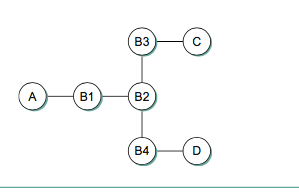
\includegraphics{ch3_15}\\
\textbf{15} Consider the arrangement of learning bridges shown in
Figure 3.49. Assuming all are initially empty, give the forwarding tables for each of the bridges B1 to B4 after the following transmissions:
\begin{enumerate}
    \item A sends to C.
    \item C sends to A.
    \item D sends to C.
\end{enumerate}
Identify ports with the unique neighbor reached directly from that port; that is, the ports for B1 are to be labeled “A” and “B2.”
\begin{solution}
    The idea is that if an incoming frame is not in the forwarding table, it is flooded, and every node in the network updates its forwarding table on the source location of the flooded packet and respond with the correct route if found. Otherwise, the incoming frame is in the forwarding table, in which case the packet is forwarded accordingly, while each switch along the way updates its forwarding table with information from frames' source  \\ 
    \textbf{Tables in the order of B1, B2, B3, B4}
    \begin{center}
        \begin{tabular}{ |c|c| } 
            Dest & Link \\ 
            \hline  
            A & A  \\ 
            C & B2 \\ 
        \end{tabular}
        \begin{tabular}{ |c|c| } 
            Dest & Link \\ 
            \hline  
            A & B1 \\ 
            C & B3 \\  
            D & B4 \\ 
        \end{tabular}
        \begin{tabular}{ |c|c| } 
            Dest & Link \\ 
            \hline  
            A & B2  \\
            C & C   \\ 
            D & B2 \\ 
        \end{tabular}
        \begin{tabular}{ |c|c| } 
            Dest & Link \\ 
            \hline  
            A & B2  \\
            D & D   \\ 
        \end{tabular}
    \end{center}
\end{solution}

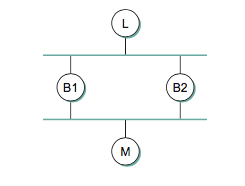
\includegraphics{ch3_19}\\
\textbf{19} Suppose learning bridges B1 and B2 form a loop as shown in Figure 3.52, and do not implement the spanning tree algorithm. Each bridge maintains a single table of $\langle address, interface\rangle$ pairs.
\begin{enumerate}
    \item What will happen if M sends to L
    \begin{solution}
        If the forwarding table have an entry for $L$ as destination, then the packets will be send accordingly. Otherwise suppose all $B1$ $B2$ and $L$s' forwarding table has no information of $M$, $M$ floods the output interface and sends packet to both $B1$ and $B2$. Each of which will loop around the $L-B2-M-B1$ cycle, one in clockwise direction and the other in counterclockwise direction .
    \end{solution}
    \item Suppose a short while later L replies to M. Give a sequence of events that leads to one packet from M and one packet from L circling the loop in opposite directions.
    \begin{solution}
        A packet sent from $L$ will cause a similar pair of packet to circulate in the cycle (in both directions). The idea is that, with learning bridges' update with packet's source node information, there maybe cases where packets are dropped (due to the fact that an entry already exists in the forwarding table). Let $AB$ be the interface connecting node $A$ and $B$
        \begin{enumerate}
            \item Suppose $L$ send a packet to $B1$, $B1$'s forwarding table is updated with entry $\langle L, B1L\rangle$
            \item Suppose that subsequently, the packet from $M$ cycling in clockwise direction is considered. Bridge $B1$ noticed that its destination $L$ is already in the forwarding table, so the packet is dropped (since we have found the route to destination $L$)
            \item Now this could similarly happen in the case where $M$ sends a packet to $B1$, and update its forwarding table with $\langle M, B1M\rangle$, in which case a packet from $L$ cycling counterclockwise encounters the $B1$, whose forwarding table has its destination node $M$, so the packet is dropped 
            \item Now, we have one remaining packet from $M$ going in counterclockwise direction and one packet from $L$ going in clockwise direction
        \end{enumerate}
    \end{solution}
\end{enumerate}



\end{document}
